\documentclass{article}
\usepackage[utf8]{inputenc}
\usepackage{graphicx}
\usepackage{titlepic}
\usepackage{hyperref}



\titlepic{
\includegraphics[width=\textwidth]{pictures/logo.jpg}}
\title{Sending data between Beckhoff PLC and Kuka Robot Controller(KRC4)}
\author{Espen Teigen }
\date{March 2019}




\begin{document}

\maketitle

    Github: https://github.com/EspenTeigen/Kuka-KR-C4-commissioning

\newpage
\section{Setting up the PLC to send and receive data with controller}
First you have to open Twincat XAE. you will get this window

\begin{figure}[!h]
    \centering
    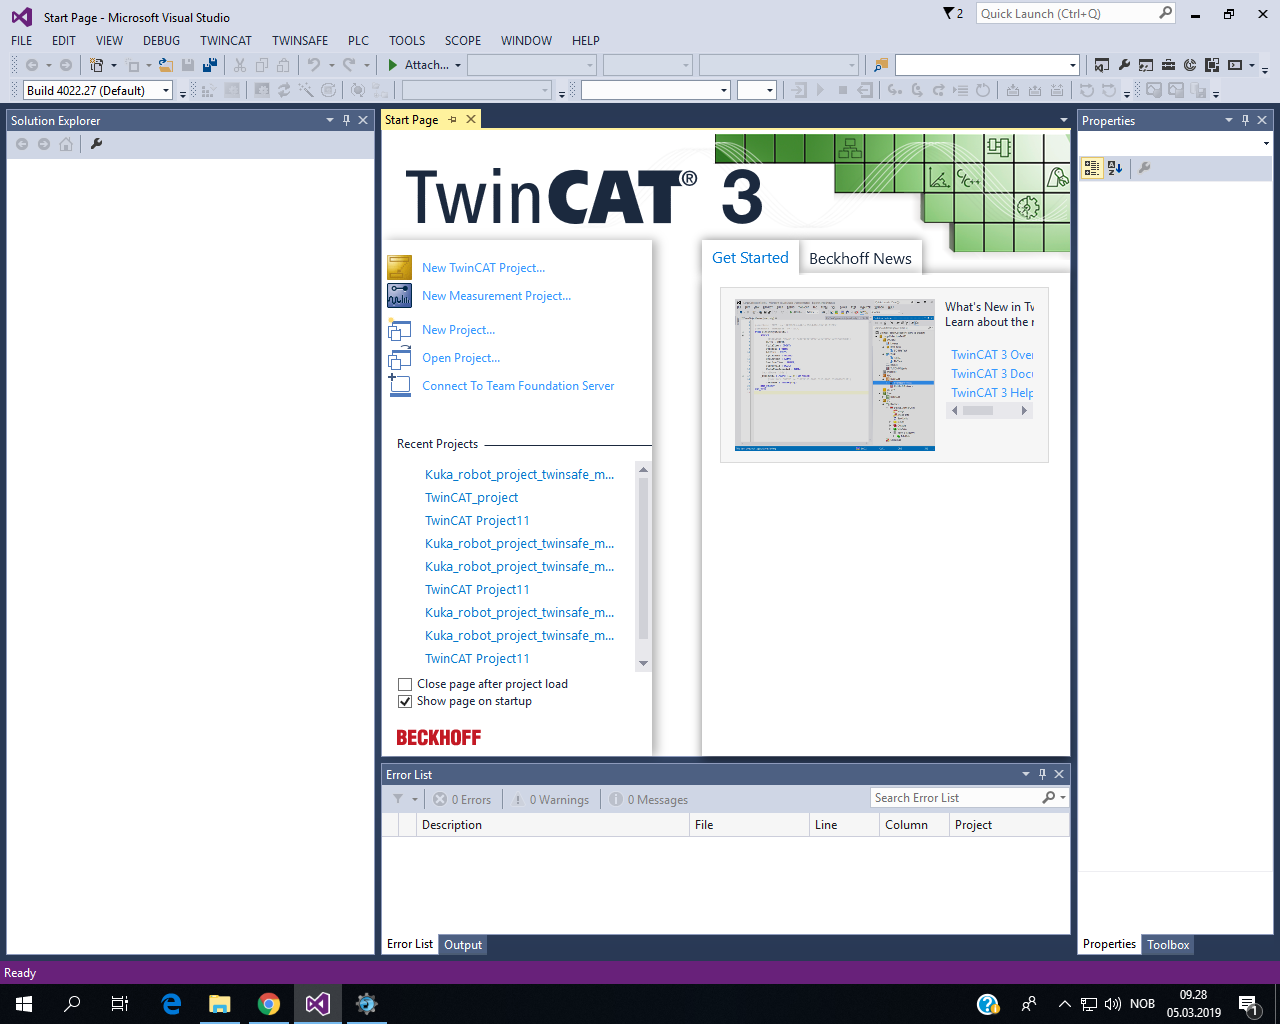
\includegraphics[width=\textwidth]{pictures/TC3_startscreen.png}
    \caption{Twincat startscreen}
    \label{fig:my_label}
\end{figure}

Select open project and in the folder TwinCAT project, you will find the microsoft visual studio solution \textbf{Kuka\_robot\_project\_twinsafe\_modbus}. If the project is not found, you can get a copy from \href{https://github.com/EspenTeigen/Kuka-KR-C4-commissioning}{\underline{github}}

\newpage
You will get this view

\begin{figure}[!h]
    \centering
    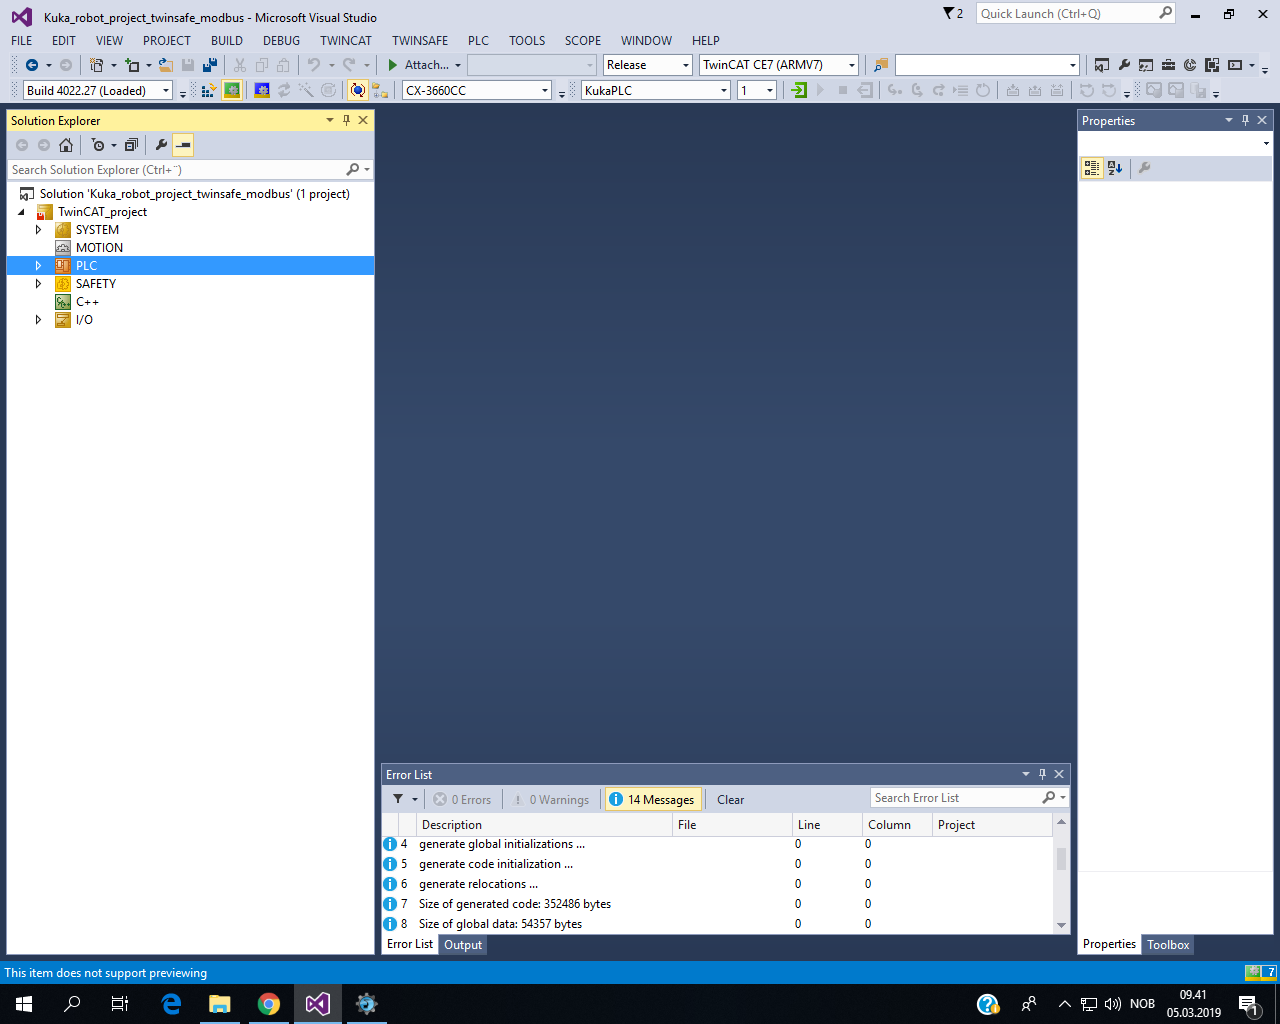
\includegraphics[width=\textwidth]{pictures/TC3_project_view.png}
    \caption{Project view}
    \label{fig:my_label2}
\end{figure}

The most interesting part off the project tree is the PLC, so expand that part. 
\newpage
We can now take a look at the different parts that are relevant for data transmission.

\begin{figure}[!h]
    \centering
    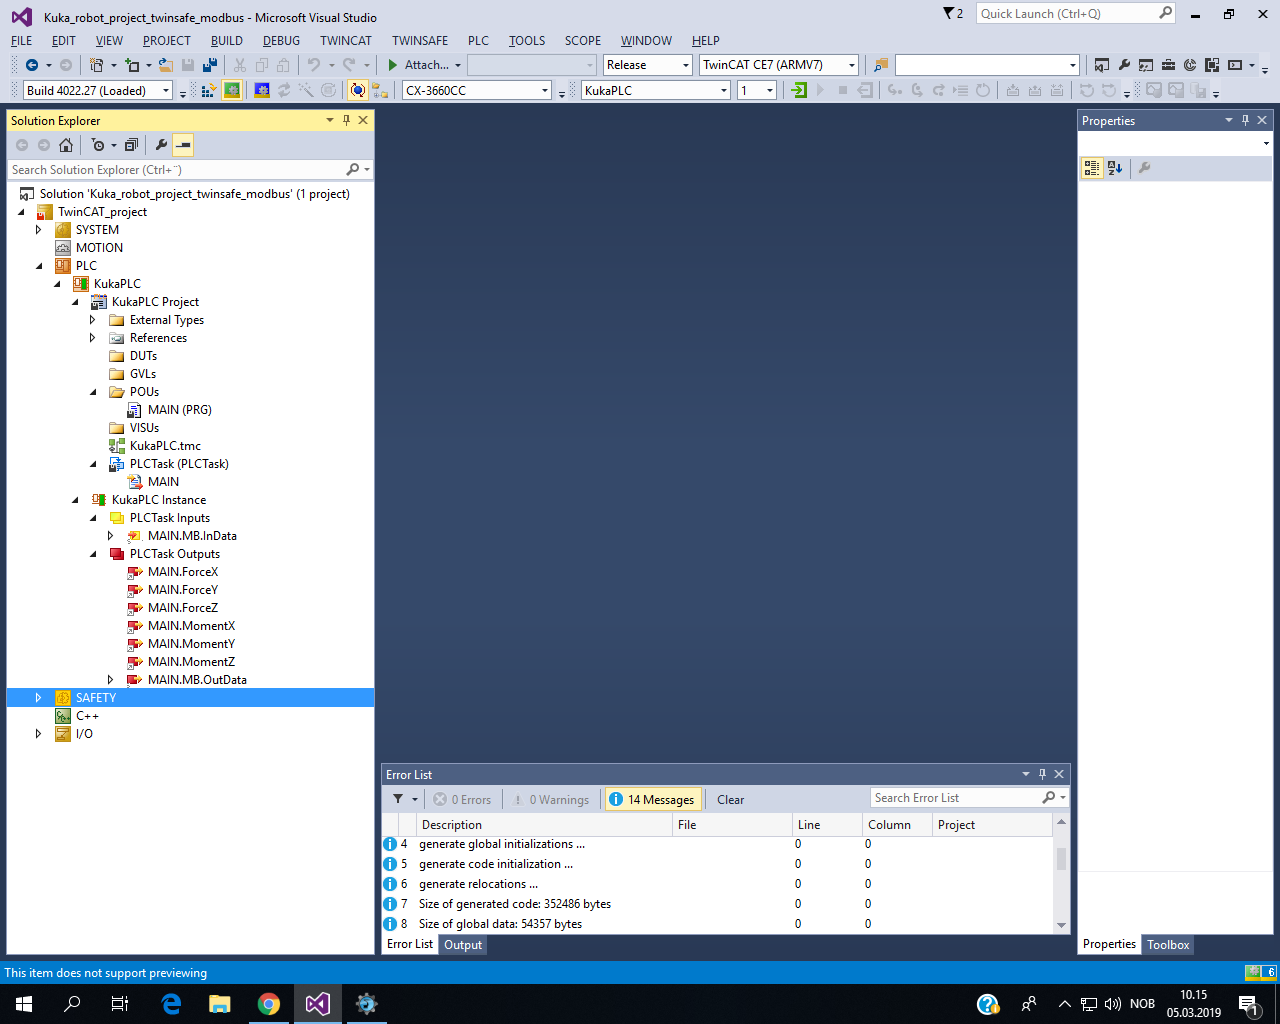
\includegraphics[width=\textwidth]{pictures/TC3_PLC_expanded.png}
    \caption{Caption}
    \label{fig:my_label}
\end{figure}

\newpage

\subsection{KukaPLC Project}
\begin{figure}[!h]
    \centering
    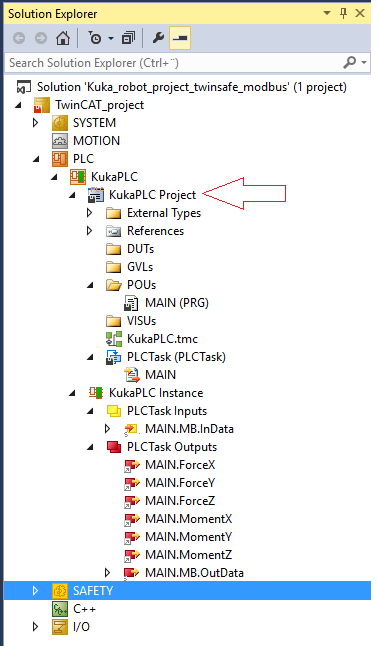
\includegraphics[scale=0.7]{pictures/TC3_KukaPLC.png}
    \caption{Caption}
    \label{fig:my_label}
\end{figure}
This is the entire PLC project, and are pre-configured to transfer data from the force-torque sensor to the robot controller. It is in this project we will set up our data transfer.  

\newpage

\subsection{POUs}
\begin{figure}[!h]
    \centering
    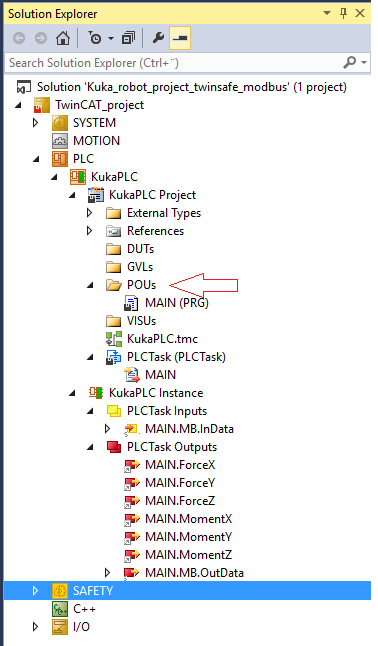
\includegraphics[scale=0.7]{pictures/TC3_POUs.png}
    \caption{}
    \label{fig:my_label}
\end{figure}

POUs are where at the programs, function blocks and functions are placed. You can chose between all the IEC 61131-3 standard programming languages. I will be using structured text. 

\newpage

\subsection{PLCTask}
\begin{figure}[!h]
    \centering
    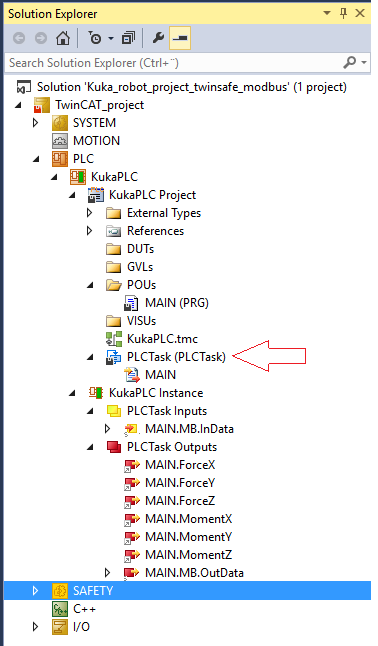
\includegraphics[scale=0.7]{pictures/TC3_PLCTask.png}
    \caption{}
    \label{fig:my_label}
\end{figure}

To understand this, i have to explain what a task is. A task is controlling the timing of how often the program should be run. You can also configure the priority of how the program should be run. If the program block is of utmost importance, and must be completed within a certain time limit, you will give it a suiting priority. 
\\
\\
PLCtask is a task that I made, and are used for this PLC. Every program that are going to be run in the PLC is timed by this task, and has to be added to it. 


\newpage

\subsection{KukaPLC instance}
\begin{figure}[!h]
    \centering
    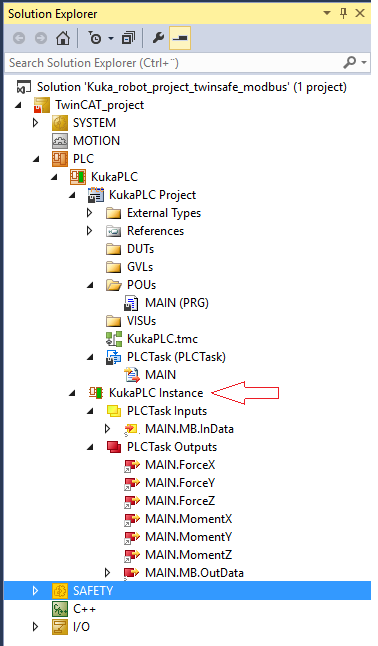
\includegraphics[scale=0.7]{pictures/TC3_KukaPLC Instance.png}
    \caption{}
    \label{fig:my_label}
\end{figure}

This is where you tie you're inputs and outputs to be transferred to and from the robot controller. When you create inputs and outputs in the PLC-program, they will end up here, and you have to link them to the module that transfer the data. Do not fret, I will describe this in a better manner later in the document. 

\newpage



\end{document}
